\subsection{Definition of the \texorpdfstring{$\chi$}{χ} Field}
  \label{subsec:definition-of-the-chi-field}

  We denote by~$\chi$ a single static pre-geometric relational substrate.
  It is not an independent primitive: the primitive of the framework is the local
  structure of admissible transitions between observable states
  (Section~\ref{subsec:minimalism-as-a-guiding-principle}), and~$\chi$ is the static
  relational structure they collectively induce, retained here as a convenient
  global description.
  The quantity~$\chi$ is not defined on a pre-existing spacetime manifold and
  does not presuppose any metric, causal, or geometric structure.
  Spacetime notions arise only as effective descriptions of the relational and
  spectral properties of~$\chi$ configurations, accessed through non-injective
  projection.

  Ontologically, $\chi$ is not a scalar order parameter and does not possess
  local values.
  Scalar order parameters arise only at the effective level, as coarse-grained
  descriptors of projected~$\chi$ configurations once a geometric regime is
  established.
  Dimensional quantities associated with length, duration, or mass arise only
  when $\chi$ configurations admit a stable geometric interpretation.

  Temporal ordering and spatial separation are not fundamental primitives.
  Temporal ordering arises from the monotone accumulation of projected spectral
  structure along the admissibility cascade
  (Section~\ref{subsec:monotonicity-and-arrow-of-time}); spatial separation
  arises from relational correlations within admissible projected configurations
  once a quasi-stable geometric regime is reached.

  The analogy with thermodynamic order parameters applies only at the effective
  level: $\chi$ itself is not an order parameter but gives rise to effective
  order parameters once projected.
  Time, space, inertial mass, gravitation, and quantum phenomena therefore emerge
  jointly as consequences of the single non-injective structure of admissible
  transitions, of which~$\chi$ is the static global representation rather than an
  independent source.

  \begin{figure}[h]
    \centering
    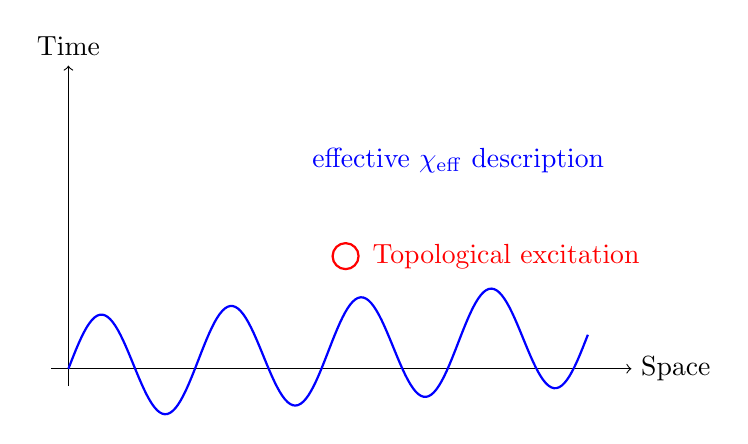
\begin{tikzpicture}[scale=1.1]
      \draw[->] (-0.2,0) -- (6.5,0) node[right]{Space};
      \draw[->] (0,-0.2) -- (0,3.5) node[above]{Time};
      \draw[thick, blue, domain=0:6, samples=200]
      plot (\x,{0.6*sin(2*pi*\x/1.5 r) + 0.4*\x/6});
      \draw[red, thick] (3.2,1.3) circle (0.15);
      \node[red, right] at (3.4,1.3) {Topological excitation};
      \node[blue] at (4.5,2.4) {effective $\chi_{\mathrm{eff}}$ description};
    \end{tikzpicture}
    \caption{Conceptual representation of Cosmochrony.
    An effective spacetime depiction of the projected scalar description
    of~$\chi$, used for visualization purposes only.
    The monotone accumulation of projected spectral structure gives rise
    to an effective temporal ordering, while localized topological excitations
    correspond to particle-like configurations in the emergent geometric regime.}
    \label{fig:chi_concept}
  \end{figure}

  Further interpretative clarifications and the fully relational formulation
  of~$\chi$ are provided in
  Appendix~\ref{subsec:nature-chi} and
  Appendix~\ref{subsec:relational-configurations}.
